\section{\textit{Oscillators}}
Los módulos más importantes de cualquier sintetizador son aquellos que son capaces de generar algún tipo de señal, sea esta audible o no. La forma más simple de generador de señal es el \textit{oscilador}, que produce una continua repetición de cambios periódicos de la señal en el tiempo. Dependiendo de la finalidad de dicha señal, en términos generales, esta puede ser \textit{de audio}, cuando su frecuencia está dentro del rango audible, o de \textit{control de voltaje}, normalmente con frecuencias por debajo del umbral de audición, y cuya función es la de modular otras señales en diversos parámetros. Esta última es la función de los llamados LFO (\textit{Low Frequency Oscillator}, por sus siglas en inglés). 

Los parámetros fundamentales de una señal periódica en cualquier sintetizador son la \textit{frecuencia} y la \textit{amplitud}. Otro parámetro, que puede ser variable o fijo, en función de su diseño, es la \textit{forma de onda}. Esta determina en alto grado el timbre o color del sonido producido, por lo que existen muchas y muy diferentes técnicas de moducación de la misma. A este respecto, cabe señalar que existen una formas de ónda básicas, por sus características matemáticas, que las convierten en básicas y comunes dentro del mundo de la síntesis sonora. Estas son la onda \textit{sinusoidal}, la \textit{triangular}, la \textit{rectangular} (también denominada \textit{pulso}), y la \textit{diente de sierra} o \textit{rampa} (fig. \ref{fig:waveforms}). No solo son posibles las transiciones entre una y otra forma de onda, como mecanismo de modulación, sino también la variación de ciertos parámetros de cada una de ellas, siendo la \textit{simetría} entre sus partes la más importante.


\begin{figure}
	\centering
	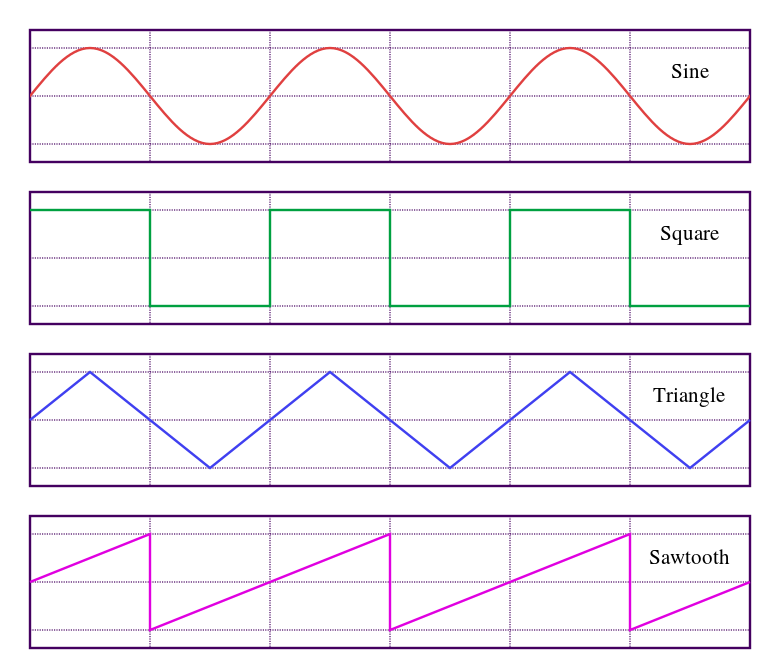
\includegraphics[width=0.7\textwidth]{images/Waveform_examples}
	\caption{Ondas periódicas simples más comunes en la síntesis sonora. (Omegatron / CC BY-SA)}
	\label{fig:waveforms}
\end{figure}

\subsection{El módulo \textit{Oscillator} en el Synthi 100}

El Synthi 100 original de EMS estaba provisto de tres osciladores \textit{sinusoidales} y \textit{de diente de sierra}, tres \textit{triangulares} y \textit{rectangulares} y, por último, tres LFO, \textit{osciladores de baja frecuencia}. El cambio introducido en el Synthi 100 de Cuenca es de gran importancia ya que pasa de 9 a 12 osciladores, cada uno de los cuales es capaz de generar cualquiera de las cuatro formas de onda, pudiéndose todos ellos commutar entre \textit{High Frecuency} y \textit{Low Frecuency} con un sencillo interruptor. A pesar de no conservar la antigua división entre \textit{Low Frecuency Oscillator} y \textit{High Frecuency Oscillator}, llama la atención que solo los tres últimos osciladores (los númerados como 10, 11 y 12) tienen una salida de voltaje, como reminiscencia de aquella división, ya que, cualquiera de las salidas del resto de osciladores (como de cualquier módulo del sintetizador) puede ser utilizada como control de voltaje gracias a la posibilidad de usar los canales de salida (\textit{Output Channels}), como \textit{busses} entre el \textit{Patchbay} de audio y el de control de voltaje (HACER REFERENCIA A LOS CANALES DE SALIDA, DONDE SE EXPLICA ESTA CARACTERÍSTICA).



\subsubsection{Los diales del módulo}

Cada oscilador del Synthi 100 de Cuenca está compuesto un interruptor LFO/HFO, denominado \textit{range}, y 7 diales (fig. \ref{fig:osciladores}).

\begin{figure}
	\centering
	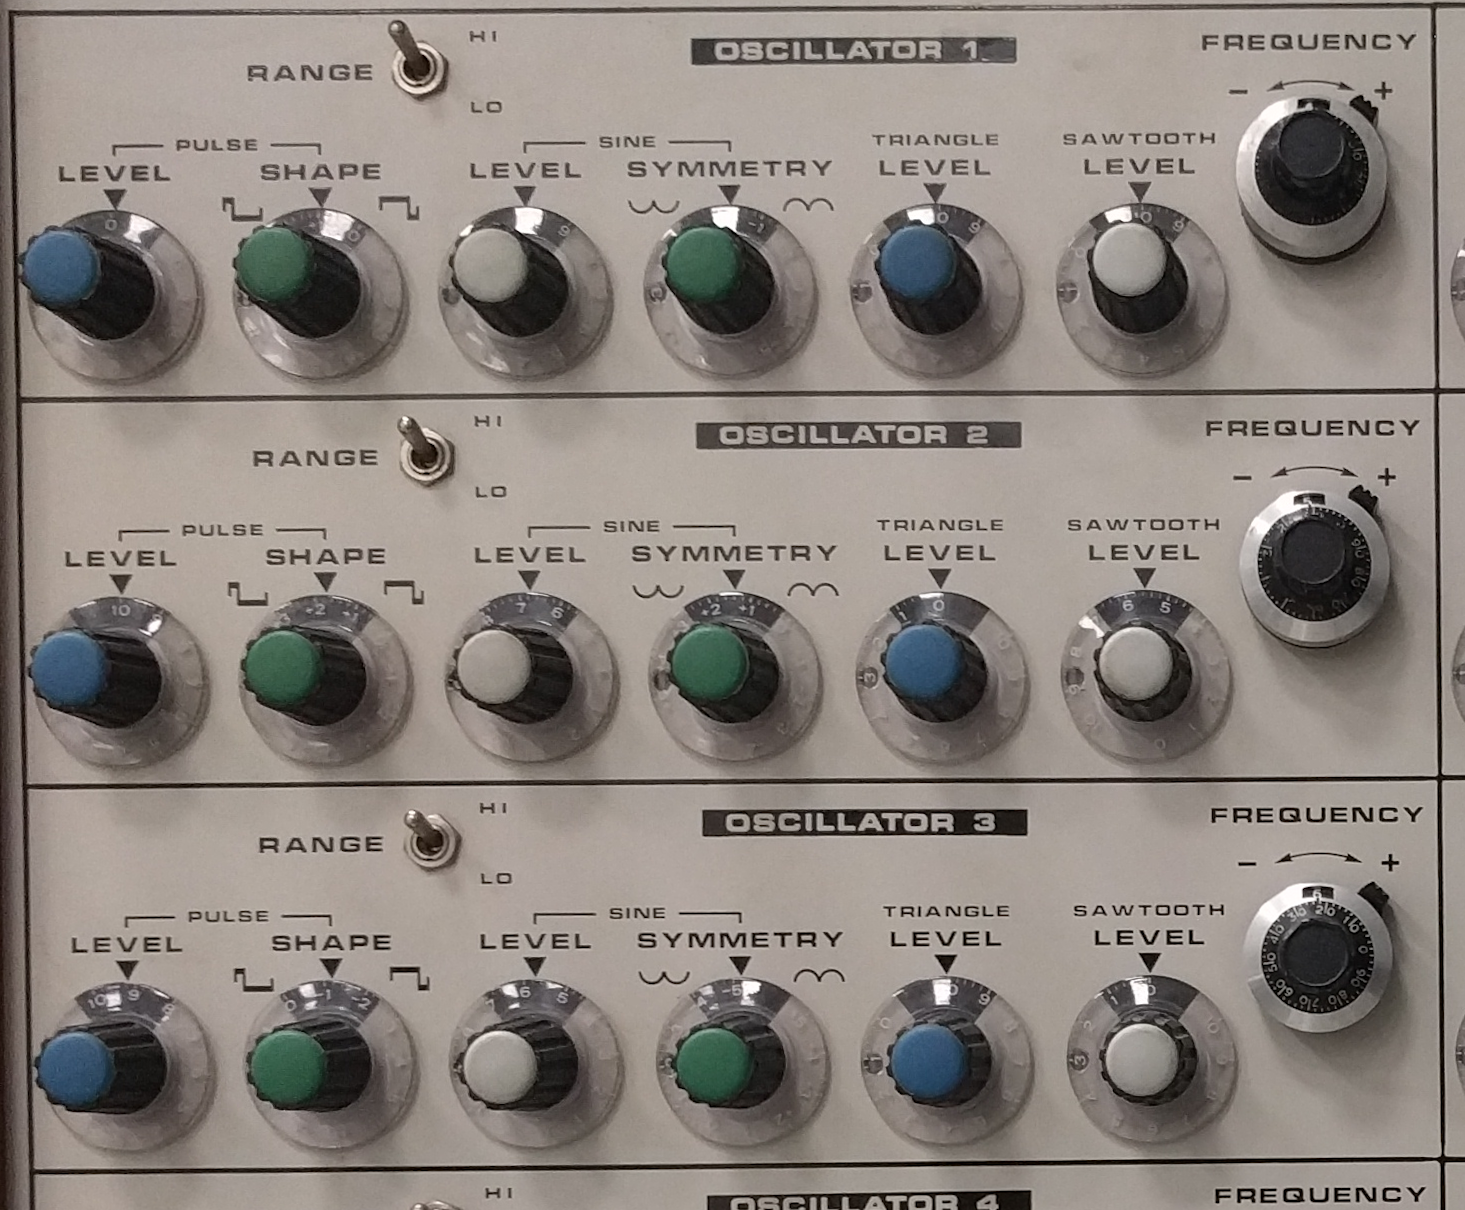
\includegraphics[width=0.7\textwidth]{images/osciladores}
	\caption{Tres de los 12 osciladores con los que cuenta el Synthi 100 del GME de Cuenca. A diferencia de versiones anteriores, este cuenta con todas cuatro formas de onda en cada uno de sus módulos, pudiendo ser utilizados tanto para bajas como altas frecuencias.}
	\label{fig:osciladores}
\end{figure}

\begin{description}
	\item[\textit{Pulse Level}] Amplitud de una señal con forma de onda \textit{rectangular}. 
	\item[\textit{Pulse Shape}] Anchura de la sección positiva de la onda. 
	\item[\textit{Sine Level}] Amplitud de la señal \textit{sinusoidal}.
	\item[\textit{Sine Symmetry}] Simetría entre las partes positiva y negativa. A menor simetría la señal adquiere progresivamente en uno de sus polos una forma más puntiaguda, rompiendo, por tanto, la simetría con el polo sinusoidal. 
	\item[\textit{Triangle Level}] Amplitud de una señal \textit{triangular}.
	\item[\textit{Sawtooth Level}] Amplitud de una señal con forma de \textit{diente de sierra}.
	\item[\textit{Frequency}] Este valor define la frecuencia de cada uno de las formas de onda. Su rango oscila entre 0.025 Hz y 500 Hz o entre 1 Hz y 10 KHz, dependiendo de si \textit{range} está en posición LFO o HFO.  
\end{description}

\subsubsection{Entradas y salidas del módulo}
Tal como se observa en las matrices de conexiones de audio y de control de voltaje, cada oscilador tiene dos salidas: una para la forma de onda sinusoidal y de diente de sierra, \textit{Sine/Saw}, y otra para la forma de onda rectangular y triangular, \textit{Pulse/Triangle}. Así, aunque todas ellas dependen de un mismo parámetro de frecuencia, sus niveles de salida y los propósitos de cada una pueden ser totalmente diversos dentro de la red de la matriz. 

Como entradas, en la matriz de \textit{control de voltaje} contamos con una por cada oscilador de control de la frecuencia, con el claro fin de permitir la técnica de síntesis por \textit{frecuencia modulada} (FM). En la matriz de \textit{señal de audio}, existe una entrada por oscilador \textit{Synchronisation inputs}, y una entrada (en los 6 primeros osciladores) de \textit{Pulse Width Modulation}, para la modulación de la forma de onda \textit{Pulse}.

\subsection{Los osciladores de la aplicación \textit{Synthi100}}
A pesar de ser uno de los módulos más elementales, es uno de los que más líneas de código tiene tras de sí, ya que aglutina a 4 osciladores, si contamos por tales cada una de las formas de onda que lo componen. \textit{Sine} está compuesto por al menos 2 Ugens de Supercollider para, haciendo \textit{morphing}, poder imitar el cambio en la simetría de la onda. Las formas de onda \textit{Triangle} y \textit{Pulse} están también formadas por dos Ugens que hacen \textit{crossfade} entre ellos para evitar el efecto de \textit{aliasing}. Son muchos Ugens en total, que pueden comprometer la eficiencia en el funcionamiento del \textit{software} en su conjunto y, por tanto, uno de los elementos a mejorar en el futuro.

A día de hoy, las entradas de audio \textit{Synchronisation inputs} y \textit{Pulse Width Modulation} están sin implementar.
